% Options for packages loaded elsewhere
\PassOptionsToPackage{unicode}{hyperref}
\PassOptionsToPackage{hyphens}{url}
%
\documentclass[
]{article}
\title{ENV 790.30 - Time Series Analysis for Energy Data \textbar{}
Spring 2021}
\usepackage{etoolbox}
\makeatletter
\providecommand{\subtitle}[1]{% add subtitle to \maketitle
  \apptocmd{\@title}{\par {\large #1 \par}}{}{}
}
\makeatother
\subtitle{Assignment 2 - Due date 01/26/22}
\author{Yared S. Asfaw}
\date{}

\usepackage{amsmath,amssymb}
\usepackage{lmodern}
\usepackage{iftex}
\ifPDFTeX
  \usepackage[T1]{fontenc}
  \usepackage[utf8]{inputenc}
  \usepackage{textcomp} % provide euro and other symbols
\else % if luatex or xetex
  \usepackage{unicode-math}
  \defaultfontfeatures{Scale=MatchLowercase}
  \defaultfontfeatures[\rmfamily]{Ligatures=TeX,Scale=1}
\fi
% Use upquote if available, for straight quotes in verbatim environments
\IfFileExists{upquote.sty}{\usepackage{upquote}}{}
\IfFileExists{microtype.sty}{% use microtype if available
  \usepackage[]{microtype}
  \UseMicrotypeSet[protrusion]{basicmath} % disable protrusion for tt fonts
}{}
\makeatletter
\@ifundefined{KOMAClassName}{% if non-KOMA class
  \IfFileExists{parskip.sty}{%
    \usepackage{parskip}
  }{% else
    \setlength{\parindent}{0pt}
    \setlength{\parskip}{6pt plus 2pt minus 1pt}}
}{% if KOMA class
  \KOMAoptions{parskip=half}}
\makeatother
\usepackage{xcolor}
\IfFileExists{xurl.sty}{\usepackage{xurl}}{} % add URL line breaks if available
\IfFileExists{bookmark.sty}{\usepackage{bookmark}}{\usepackage{hyperref}}
\hypersetup{
  pdftitle={ENV 790.30 - Time Series Analysis for Energy Data \textbar{} Spring 2021},
  pdfauthor={Yared S. Asfaw},
  hidelinks,
  pdfcreator={LaTeX via pandoc}}
\urlstyle{same} % disable monospaced font for URLs
\usepackage[margin=2.54cm]{geometry}
\usepackage{color}
\usepackage{fancyvrb}
\newcommand{\VerbBar}{|}
\newcommand{\VERB}{\Verb[commandchars=\\\{\}]}
\DefineVerbatimEnvironment{Highlighting}{Verbatim}{commandchars=\\\{\}}
% Add ',fontsize=\small' for more characters per line
\usepackage{framed}
\definecolor{shadecolor}{RGB}{248,248,248}
\newenvironment{Shaded}{\begin{snugshade}}{\end{snugshade}}
\newcommand{\AlertTok}[1]{\textcolor[rgb]{0.94,0.16,0.16}{#1}}
\newcommand{\AnnotationTok}[1]{\textcolor[rgb]{0.56,0.35,0.01}{\textbf{\textit{#1}}}}
\newcommand{\AttributeTok}[1]{\textcolor[rgb]{0.77,0.63,0.00}{#1}}
\newcommand{\BaseNTok}[1]{\textcolor[rgb]{0.00,0.00,0.81}{#1}}
\newcommand{\BuiltInTok}[1]{#1}
\newcommand{\CharTok}[1]{\textcolor[rgb]{0.31,0.60,0.02}{#1}}
\newcommand{\CommentTok}[1]{\textcolor[rgb]{0.56,0.35,0.01}{\textit{#1}}}
\newcommand{\CommentVarTok}[1]{\textcolor[rgb]{0.56,0.35,0.01}{\textbf{\textit{#1}}}}
\newcommand{\ConstantTok}[1]{\textcolor[rgb]{0.00,0.00,0.00}{#1}}
\newcommand{\ControlFlowTok}[1]{\textcolor[rgb]{0.13,0.29,0.53}{\textbf{#1}}}
\newcommand{\DataTypeTok}[1]{\textcolor[rgb]{0.13,0.29,0.53}{#1}}
\newcommand{\DecValTok}[1]{\textcolor[rgb]{0.00,0.00,0.81}{#1}}
\newcommand{\DocumentationTok}[1]{\textcolor[rgb]{0.56,0.35,0.01}{\textbf{\textit{#1}}}}
\newcommand{\ErrorTok}[1]{\textcolor[rgb]{0.64,0.00,0.00}{\textbf{#1}}}
\newcommand{\ExtensionTok}[1]{#1}
\newcommand{\FloatTok}[1]{\textcolor[rgb]{0.00,0.00,0.81}{#1}}
\newcommand{\FunctionTok}[1]{\textcolor[rgb]{0.00,0.00,0.00}{#1}}
\newcommand{\ImportTok}[1]{#1}
\newcommand{\InformationTok}[1]{\textcolor[rgb]{0.56,0.35,0.01}{\textbf{\textit{#1}}}}
\newcommand{\KeywordTok}[1]{\textcolor[rgb]{0.13,0.29,0.53}{\textbf{#1}}}
\newcommand{\NormalTok}[1]{#1}
\newcommand{\OperatorTok}[1]{\textcolor[rgb]{0.81,0.36,0.00}{\textbf{#1}}}
\newcommand{\OtherTok}[1]{\textcolor[rgb]{0.56,0.35,0.01}{#1}}
\newcommand{\PreprocessorTok}[1]{\textcolor[rgb]{0.56,0.35,0.01}{\textit{#1}}}
\newcommand{\RegionMarkerTok}[1]{#1}
\newcommand{\SpecialCharTok}[1]{\textcolor[rgb]{0.00,0.00,0.00}{#1}}
\newcommand{\SpecialStringTok}[1]{\textcolor[rgb]{0.31,0.60,0.02}{#1}}
\newcommand{\StringTok}[1]{\textcolor[rgb]{0.31,0.60,0.02}{#1}}
\newcommand{\VariableTok}[1]{\textcolor[rgb]{0.00,0.00,0.00}{#1}}
\newcommand{\VerbatimStringTok}[1]{\textcolor[rgb]{0.31,0.60,0.02}{#1}}
\newcommand{\WarningTok}[1]{\textcolor[rgb]{0.56,0.35,0.01}{\textbf{\textit{#1}}}}
\usepackage{graphicx}
\makeatletter
\def\maxwidth{\ifdim\Gin@nat@width>\linewidth\linewidth\else\Gin@nat@width\fi}
\def\maxheight{\ifdim\Gin@nat@height>\textheight\textheight\else\Gin@nat@height\fi}
\makeatother
% Scale images if necessary, so that they will not overflow the page
% margins by default, and it is still possible to overwrite the defaults
% using explicit options in \includegraphics[width, height, ...]{}
\setkeys{Gin}{width=\maxwidth,height=\maxheight,keepaspectratio}
% Set default figure placement to htbp
\makeatletter
\def\fps@figure{htbp}
\makeatother
\setlength{\emergencystretch}{3em} % prevent overfull lines
\providecommand{\tightlist}{%
  \setlength{\itemsep}{0pt}\setlength{\parskip}{0pt}}
\setcounter{secnumdepth}{-\maxdimen} % remove section numbering
\ifLuaTeX
  \usepackage{selnolig}  % disable illegal ligatures
\fi

\begin{document}
\maketitle

\hypertarget{submission-instructions}{%
\subsection{Submission Instructions}\label{submission-instructions}}

You should open the .rmd file corresponding to this assignment on
RStudio. The file is available on our class repository on Github.

Once you have the file open on your local machine the first thing you
will do is change ``Student Name'' on line 4 with your name. Then you
will start working through the assignment by \textbf{creating code and
output} that answer each question. Be sure to use this assignment
document. Your report should contain the answer to each question and any
plots/tables you obtained (when applicable).

When you have completed the assignment, \textbf{Knit} the text and code
into a single PDF file. Rename the pdf file such that it includes your
first and last name (e.g., ``LuanaLima\_TSA\_A02\_Sp22.Rmd''). Submit
this pdf using Sakai.

\hypertarget{r-packages}{%
\subsection{R packages}\label{r-packages}}

R packages needed for this assignment:``forecast'',``tseries'', and
``dplyr''. Install these packages, if you haven't done yet. Do not
forget to load them before running your script, since they are NOT
default packages.

\hypertarget{data-set-information}{%
\subsection{Data set information}\label{data-set-information}}

Consider the data provided in the spreadsheet
``Table\_10.1\_Renewable\_Energy\_Production\_
and\_Consumption\_by\_Source.xlsx'' on our \textbf{Data} folder. The
data comes from the US Energy Information and Administration and
corresponds to the January 2022 Monthly Energy Review. The spreadsheet
is ready to be used. Use the command \(read.table()\) to import the data
in R or \(panda.read\_excel()\) in Python (note that you will need to
import pandas package). \}

\begin{Shaded}
\begin{Highlighting}[]
\CommentTok{\#Importing the data set}
\FunctionTok{library}\NormalTok{(openxlsx)}
\NormalTok{USEne.data }\OtherTok{\textless{}{-}} \FunctionTok{read.xlsx}\NormalTok{(}\StringTok{"./Data/Raw/Table\_10.1\_Ren.\_Energy\_PC.\_by\_Source.xlsx"}\NormalTok{, }\AttributeTok{startRow=}\DecValTok{11}\NormalTok{)}
\end{Highlighting}
\end{Shaded}

\hypertarget{question-1}{%
\subsection{Question 1}\label{question-1}}

You will work only with the following columns: Total Biomass Energy
Production, Total Renewable Energy Production, Hydroelectric Power
Consumption. Create a data frame structure with these three time series
only. Use the command head() to verify your data.

\begin{Shaded}
\begin{Highlighting}[]
\CommentTok{\#Create data frame with the three variables}
\NormalTok{selected\_var.df }\OtherTok{\textless{}{-}} \FunctionTok{data.frame}\NormalTok{(USEne.data [,}\FunctionTok{c}\NormalTok{(}\DecValTok{1}\NormalTok{,}\DecValTok{4}\NormalTok{,}\DecValTok{5}\NormalTok{,}\DecValTok{6}\NormalTok{)])}

\FunctionTok{is.data.frame}\NormalTok{(selected\_var.df)}
\end{Highlighting}
\end{Shaded}

\begin{verbatim}
## [1] TRUE
\end{verbatim}

\begin{Shaded}
\begin{Highlighting}[]
\FunctionTok{head}\NormalTok{(selected\_var.df)}
\end{Highlighting}
\end{Shaded}

\begin{verbatim}
##   Month Total.Biomass.Energy.Production Total.Renewable.Energy.Production
## 1    NA                  (Trillion Btu)                    (Trillion Btu)
## 2 26665                         129.787                           403.981
## 3 26696                         117.338                             360.9
## 4 26724                         129.938                           400.161
## 5 26755                         125.636                            380.47
## 6 26785                         129.834                           392.141
##   Hydroelectric.Power.Consumption
## 1                  (Trillion Btu)
## 2                         272.703
## 3                         242.199
## 4                          268.81
## 5                         253.185
## 6                          260.77
\end{verbatim}

\begin{Shaded}
\begin{Highlighting}[]
\NormalTok{selected\_var.df.data }\OtherTok{\textless{}{-}}\NormalTok{ selected\_var.df[}\SpecialCharTok{{-}}\DecValTok{1}\NormalTok{,]}
\CommentTok{\#To remove the row that contains the unit of measurement  }
\FunctionTok{is.data.frame}\NormalTok{(selected\_var.df.data)}
\end{Highlighting}
\end{Shaded}

\begin{verbatim}
## [1] TRUE
\end{verbatim}

\begin{Shaded}
\begin{Highlighting}[]
\FunctionTok{head}\NormalTok{(selected\_var.df.data)}
\end{Highlighting}
\end{Shaded}

\begin{verbatim}
##   Month Total.Biomass.Energy.Production Total.Renewable.Energy.Production
## 2 26665                         129.787                           403.981
## 3 26696                         117.338                             360.9
## 4 26724                         129.938                           400.161
## 5 26755                         125.636                            380.47
## 6 26785                         129.834                           392.141
## 7 26816                         125.611                           377.232
##   Hydroelectric.Power.Consumption
## 2                         272.703
## 3                         242.199
## 4                          268.81
## 5                         253.185
## 6                          260.77
## 7                         249.859
\end{verbatim}

\begin{Shaded}
\begin{Highlighting}[]
\CommentTok{\#changing the class or type of the selected variables from character to numeric}
\CommentTok{\#For simplicity let us rename the columns}
\FunctionTok{colnames}\NormalTok{(selected\_var.df.data) }\OtherTok{\textless{}{-}} \FunctionTok{c}\NormalTok{(}\StringTok{"month"}\NormalTok{, }\StringTok{"biomass"}\NormalTok{,}\StringTok{"renewable"}\NormalTok{, }\StringTok{"hydro"}\NormalTok{)}

\NormalTok{selected\_var.df.data}\SpecialCharTok{$}\NormalTok{biomass }\OtherTok{\textless{}{-}} \FunctionTok{as.numeric}\NormalTok{(selected\_var.df.data}\SpecialCharTok{$}\NormalTok{biomass)}

\NormalTok{selected\_var.df.data}\SpecialCharTok{$}\NormalTok{renewable }\OtherTok{\textless{}{-}} \FunctionTok{as.numeric}\NormalTok{(selected\_var.df.data}\SpecialCharTok{$}\NormalTok{renewable)}

\NormalTok{selected\_var.df.data}\SpecialCharTok{$}\NormalTok{hydro }\OtherTok{\textless{}{-}} \FunctionTok{as.numeric}\NormalTok{(selected\_var.df.data}\SpecialCharTok{$}\NormalTok{hydro)}
\end{Highlighting}
\end{Shaded}

\hypertarget{question-2}{%
\subsection{Question 2}\label{question-2}}

Transform your data frame in a time series object and specify the
starting point and frequency of the time series using the function ts().

\begin{Shaded}
\begin{Highlighting}[]
\CommentTok{\#Time series object of Total Biomass Energy Production}
\NormalTok{ts.biomass }\OtherTok{\textless{}{-}} \FunctionTok{ts}\NormalTok{(selected\_var.df.data}\SpecialCharTok{$}\NormalTok{biomass, }\AttributeTok{start =} \FunctionTok{c}\NormalTok{(}\DecValTok{1973}\NormalTok{, }\DecValTok{1}\NormalTok{), }\AttributeTok{frequency =} \DecValTok{12}\NormalTok{)}

\CommentTok{\#Time series object of Total Renewable Energy Production}
\NormalTok{ts.Re\_energy }\OtherTok{\textless{}{-}} \FunctionTok{ts}\NormalTok{(selected\_var.df.data}\SpecialCharTok{$}\NormalTok{renewable, }\AttributeTok{start =} \FunctionTok{c}\NormalTok{(}\DecValTok{1973}\NormalTok{, }\DecValTok{1}\NormalTok{), }\AttributeTok{frequency =} \DecValTok{12}\NormalTok{)}

\CommentTok{\#Time series object of Hydroelectric Power Consumption }
\NormalTok{ts.hyd\_usage }\OtherTok{\textless{}{-}} \FunctionTok{ts}\NormalTok{(selected\_var.df.data}\SpecialCharTok{$}\NormalTok{hydro, }\AttributeTok{start =} \FunctionTok{c}\NormalTok{(}\DecValTok{1973}\NormalTok{, }\DecValTok{1}\NormalTok{), }\AttributeTok{frequency =} \DecValTok{12}\NormalTok{)}
\end{Highlighting}
\end{Shaded}

\hypertarget{question-3}{%
\subsection{Question 3}\label{question-3}}

Compute mean and standard deviation for these three series.

\begin{Shaded}
\begin{Highlighting}[]
\FunctionTok{mean}\NormalTok{(ts.biomass) }
\end{Highlighting}
\end{Shaded}

\begin{verbatim}
## [1] 273.7839
\end{verbatim}

\hypertarget{the-mean-of-the-total-biomass-energy-production-for-the-given-time-series-is-273.78-trillion-btu.}{%
\subsubsection{The mean of the total biomass energy production for the
given time series is 273.78 Trillion
Btu.}\label{the-mean-of-the-total-biomass-energy-production-for-the-given-time-series-is-273.78-trillion-btu.}}

\begin{Shaded}
\begin{Highlighting}[]
\FunctionTok{sd}\NormalTok{(ts.biomass) }
\end{Highlighting}
\end{Shaded}

\begin{verbatim}
## [1] 89.42852
\end{verbatim}

\hypertarget{the-standard-deviation-of-the-total-biomass-energy-production-for-the-given-time-series-is-89.43-trillion-btu.}{%
\subsubsection{The standard deviation of the total biomass energy
production for the given time series is 89.43 Trillion
Btu.}\label{the-standard-deviation-of-the-total-biomass-energy-production-for-the-given-time-series-is-89.43-trillion-btu.}}

\begin{Shaded}
\begin{Highlighting}[]
\FunctionTok{mean}\NormalTok{(ts.Re\_energy)}
\end{Highlighting}
\end{Shaded}

\begin{verbatim}
## [1] 581.1708
\end{verbatim}

\hypertarget{the-mean-of-the-total-renewable-energy-production-for-the-given-time-series-is-581.17-trillion-btu.}{%
\subsubsection{The mean of the total renewable energy production for the
given time series is 581.17 Trillion
Btu.}\label{the-mean-of-the-total-renewable-energy-production-for-the-given-time-series-is-581.17-trillion-btu.}}

\begin{Shaded}
\begin{Highlighting}[]
\FunctionTok{sd}\NormalTok{(ts.Re\_energy)}
\end{Highlighting}
\end{Shaded}

\begin{verbatim}
## [1] 177.5607
\end{verbatim}

\hypertarget{the-standard-deviation-of-the-total-renewable-energy-production-for-the-given-time-series-is-177.56-trillion-btu.}{%
\subsubsection{The standard deviation of the total renewable energy
production for the given time series is 177.56 Trillion
Btu.}\label{the-standard-deviation-of-the-total-renewable-energy-production-for-the-given-time-series-is-177.56-trillion-btu.}}

\begin{Shaded}
\begin{Highlighting}[]
\FunctionTok{mean}\NormalTok{(ts.hyd\_usage) }
\end{Highlighting}
\end{Shaded}

\begin{verbatim}
## [1] 235.9653
\end{verbatim}

\hypertarget{the-mean-of-the-hydroelectric-power-consumption-for-the-given-time-series-is-235.97-trillion-btu.}{%
\subsubsection{The mean of the hydroelectric power consumption for the
given time series is 235.97 Trillion
Btu.}\label{the-mean-of-the-hydroelectric-power-consumption-for-the-given-time-series-is-235.97-trillion-btu.}}

\begin{Shaded}
\begin{Highlighting}[]
\FunctionTok{sd}\NormalTok{(ts.hyd\_usage) }
\end{Highlighting}
\end{Shaded}

\begin{verbatim}
## [1] 44.01749
\end{verbatim}

\hypertarget{the-standard-deviation-of-the-total-biomass-energy-production-for-the-given-time-series-is-44.02-trillion-btu.}{%
\paragraph{The standard deviation of the total biomass energy production
for the given time series is 44.02 Trillion
Btu.}\label{the-standard-deviation-of-the-total-biomass-energy-production-for-the-given-time-series-is-44.02-trillion-btu.}}

\hypertarget{question-4}{%
\subsection{Question 4}\label{question-4}}

Display and interpret the time series plot for each of these variables.
Try to make your plot as informative as possible by writing titles,
labels, etc. For each plot add a horizontal line at the mean of each
series in a different color.

\begin{Shaded}
\begin{Highlighting}[]
\CommentTok{\# Time series plot of Total Biomass Energy Production}
\FunctionTok{plot}\NormalTok{(ts.biomass,}\AttributeTok{type=}\StringTok{"l"}\NormalTok{,}\AttributeTok{col=}\StringTok{"blue"}\NormalTok{,}\AttributeTok{xlab=}\StringTok{"Year"}\NormalTok{,}\AttributeTok{ylab=}\StringTok{"BEP [Trillion Btu]"}\NormalTok{,}
\AttributeTok{main=}\StringTok{"U.S.Total Biomass Energy Production (BEP)"}\NormalTok{)}
\FunctionTok{abline}\NormalTok{(}\AttributeTok{h=}\FunctionTok{mean}\NormalTok{(ts.biomass),}\AttributeTok{col=}\StringTok{"red"}\NormalTok{) }
\end{Highlighting}
\end{Shaded}

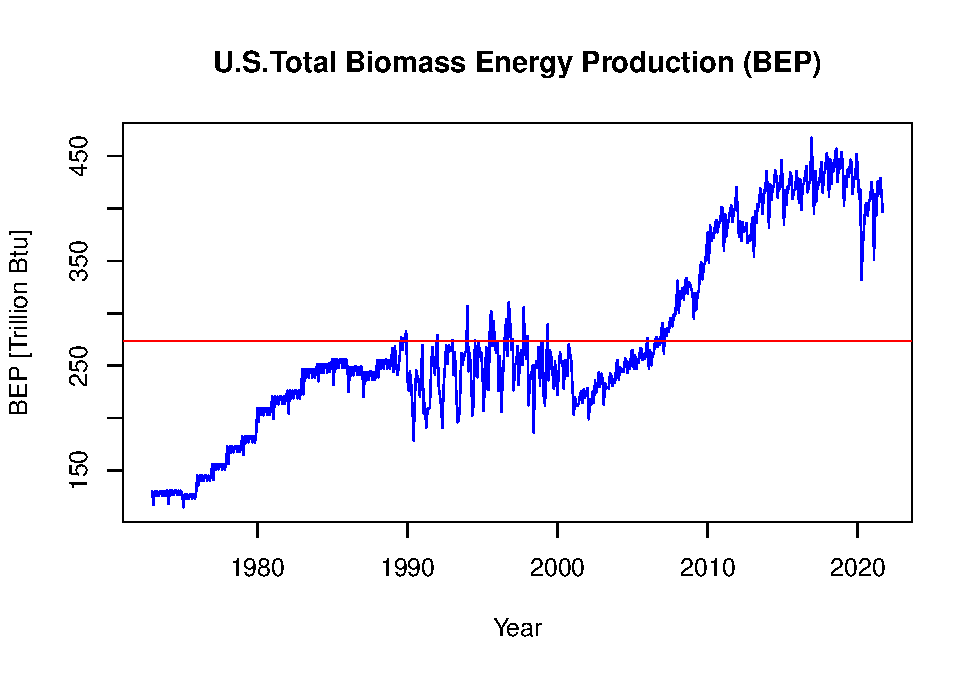
\includegraphics{YaredAsfaw_TSA_A02_Sp22_files/figure-latex/unnamed-chunk-11-1.pdf}

\begin{Shaded}
\begin{Highlighting}[]
\CommentTok{\# Time series plot of Total Renewable Energy Production}
\FunctionTok{plot}\NormalTok{(ts.Re\_energy,}\AttributeTok{type=}\StringTok{"l"}\NormalTok{,}\AttributeTok{col=}\StringTok{"green"}\NormalTok{,}\AttributeTok{xlab=}\StringTok{"Year"}\NormalTok{,}\AttributeTok{ylab=}\StringTok{"REP [Trillion Btu]"}\NormalTok{,}
\AttributeTok{main=}\StringTok{"U.S. Total Renewable Energy Production (REP)"}\NormalTok{) }
\FunctionTok{abline}\NormalTok{(}\AttributeTok{h=}\FunctionTok{mean}\NormalTok{(ts.Re\_energy),}\AttributeTok{col=}\StringTok{"red"}\NormalTok{)}
\end{Highlighting}
\end{Shaded}

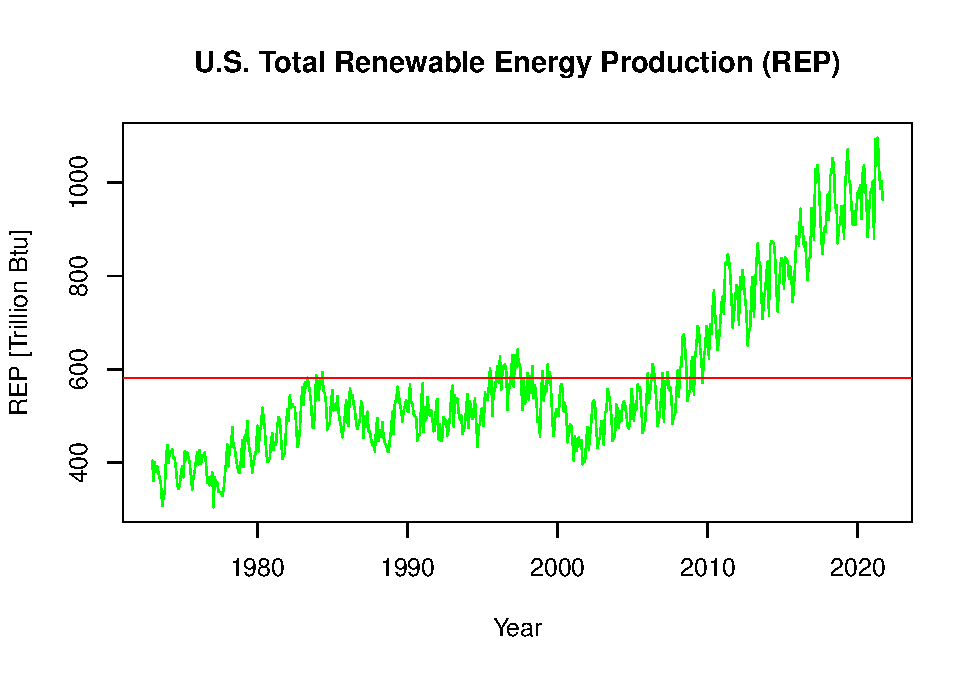
\includegraphics{YaredAsfaw_TSA_A02_Sp22_files/figure-latex/unnamed-chunk-12-1.pdf}

\begin{Shaded}
\begin{Highlighting}[]
\CommentTok{\# Time series plot of Hydroelectric Power Consumption}
\FunctionTok{plot}\NormalTok{(ts.hyd\_usage,}\AttributeTok{type=}\StringTok{"l"}\NormalTok{,}\AttributeTok{col=}\StringTok{"red"}\NormalTok{,}\AttributeTok{xlab=}\StringTok{"Year"}\NormalTok{,}\AttributeTok{ylab=}\StringTok{"HEPC [Trillion Btu]"}\NormalTok{,}
\AttributeTok{main=}\StringTok{"U.S. Hydroelectric Power Consumption (HEPC)"}\NormalTok{)}
\FunctionTok{abline}\NormalTok{(}\AttributeTok{h=}\FunctionTok{mean}\NormalTok{(ts.hyd\_usage),}\AttributeTok{col=}\StringTok{"blue"}\NormalTok{)}
\end{Highlighting}
\end{Shaded}

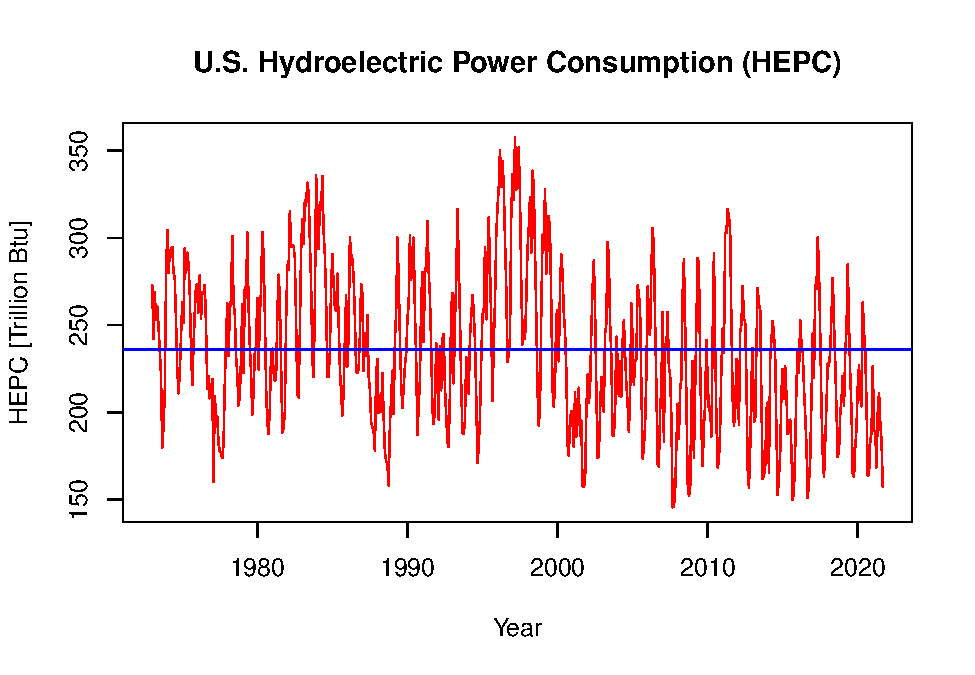
\includegraphics{YaredAsfaw_TSA_A02_Sp22_files/figure-latex/unnamed-chunk-13-1.pdf}

\hypertarget{question-5}{%
\subsection{Question 5}\label{question-5}}

Are they significantly correlated? Explain your answer.

\begin{Shaded}
\begin{Highlighting}[]
\FunctionTok{cor}\NormalTok{(selected\_var.df.data [,}\DecValTok{2}\SpecialCharTok{:}\DecValTok{4}\NormalTok{])  }
\end{Highlighting}
\end{Shaded}

\begin{verbatim}
##              biomass   renewable       hydro
## biomass    1.0000000  0.92328377 -0.28049970
## renewable  0.9232838  1.00000000 -0.05680651
## hydro     -0.2804997 -0.05680651  1.00000000
\end{verbatim}

\hypertarget{correlation-table-of-the-three-variables.-another-option-is-shown-below-separately-doing-the-correlation-between-pairs-of-variables.}{%
\subsubsection{Correlation table of the three variables. Another option
is shown below, separately doing the correlation between pairs of
variables.}\label{correlation-table-of-the-three-variables.-another-option-is-shown-below-separately-doing-the-correlation-between-pairs-of-variables.}}

\begin{Shaded}
\begin{Highlighting}[]
\FunctionTok{cor}\NormalTok{(selected\_var.df.data}\SpecialCharTok{$}\NormalTok{biomass, selected\_var.df.data}\SpecialCharTok{$}\NormalTok{renewable)  }
\end{Highlighting}
\end{Shaded}

\begin{verbatim}
## [1] 0.9232838
\end{verbatim}

\hypertarget{the-total-biomass-energy-production-and-the-total-renewable-energy-production-are-highly-significantly-correlated-with-a-correlation-coefficient-of-0.92.}{%
\subsubsection{The total biomass energy production and the total
renewable energy production are highly significantly correlated with a
correlation coefficient of
0.92.}\label{the-total-biomass-energy-production-and-the-total-renewable-energy-production-are-highly-significantly-correlated-with-a-correlation-coefficient-of-0.92.}}

\begin{Shaded}
\begin{Highlighting}[]
\FunctionTok{cor}\NormalTok{(selected\_var.df.data}\SpecialCharTok{$}\NormalTok{biomass, selected\_var.df.data}\SpecialCharTok{$}\NormalTok{hydro) }
\end{Highlighting}
\end{Shaded}

\begin{verbatim}
## [1] -0.2804997
\end{verbatim}

\hypertarget{the-total-biomass-energy-production-and-the-hydroelectric-power-consumption-are-slightly-negatively-correlated-with-a-correlation-coefficient-of--0.2805.-that-means-an-increase-in-biomass-energy-production-will-decrease-the-hydroelectric-power-consumption-by-28.05.}{%
\subsubsection{The total biomass energy production and the hydroelectric
power consumption are slightly negatively correlated with a correlation
coefficient of -0.2805. That means an increase in biomass energy
production will decrease the hydroelectric power consumption by
28.05\%.}\label{the-total-biomass-energy-production-and-the-hydroelectric-power-consumption-are-slightly-negatively-correlated-with-a-correlation-coefficient-of--0.2805.-that-means-an-increase-in-biomass-energy-production-will-decrease-the-hydroelectric-power-consumption-by-28.05.}}

\begin{Shaded}
\begin{Highlighting}[]
\FunctionTok{cor}\NormalTok{(selected\_var.df.data}\SpecialCharTok{$}\NormalTok{renewable, selected\_var.df.data}\SpecialCharTok{$}\NormalTok{hydro)  }
\end{Highlighting}
\end{Shaded}

\begin{verbatim}
## [1] -0.05680651
\end{verbatim}

\hypertarget{the-total-renewable-energy-production-and-hydroelectric-power-consumption-show-a-very-small-negative-or-almost-no-correlation-with-a-correlation-coefficient-of--0.057.}{%
\subsubsection{The total renewable energy production and hydroelectric
power consumption show a very small negative or almost no correlation
with a correlation coefficient of
-0.057.}\label{the-total-renewable-energy-production-and-hydroelectric-power-consumption-show-a-very-small-negative-or-almost-no-correlation-with-a-correlation-coefficient-of--0.057.}}

\hypertarget{question-6}{%
\subsection{Question 6}\label{question-6}}

Compute the autocorrelation function from lag 1 up to lag 40 for these
three variables. What can you say about these plots? Do the three of
them have the same behavior?

\begin{Shaded}
\begin{Highlighting}[]
\NormalTok{acf\_ts.biomass }\OtherTok{\textless{}{-}} \FunctionTok{acf}\NormalTok{(selected\_var.df.data}\SpecialCharTok{$}\NormalTok{biomass, }\AttributeTok{lag.max =} \DecValTok{40}\NormalTok{, }\AttributeTok{plot=}\ConstantTok{TRUE}\NormalTok{)  }
\end{Highlighting}
\end{Shaded}

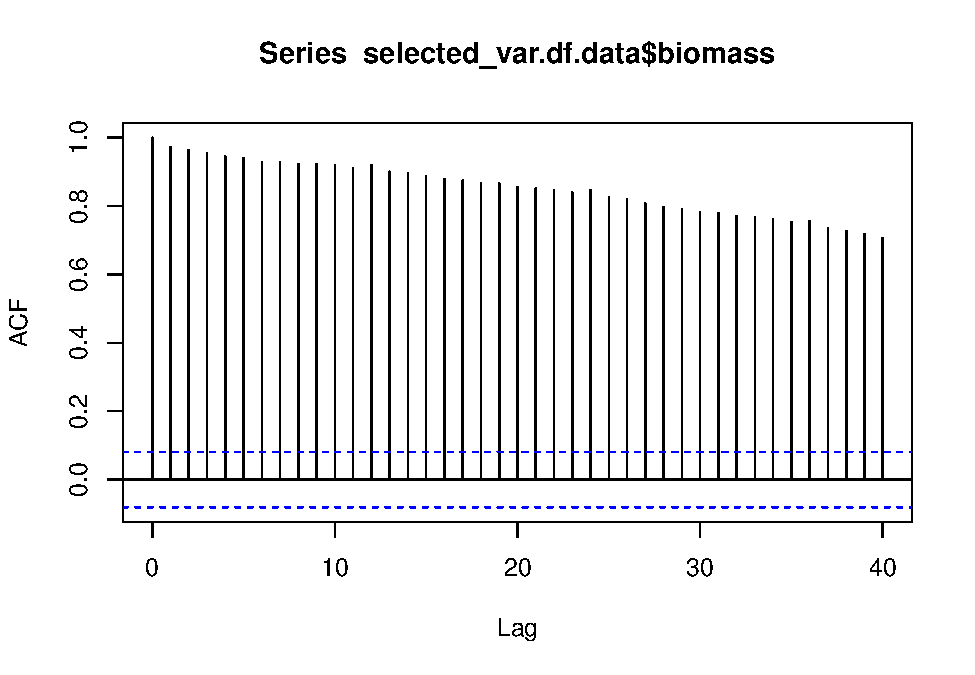
\includegraphics{YaredAsfaw_TSA_A02_Sp22_files/figure-latex/unnamed-chunk-18-1.pdf}

\hypertarget{there-is-a-significant-correlation-among-the-observations-of-the-total-biomass-energy-production-at-different-time-series.-however-this-correlation-show-a-decreasing-trend-as-the-time-lag-increases.}{%
\subsubsection{There is a significant correlation among the observations
of the total biomass energy production at different time series.
However, this correlation show a decreasing trend as the time lag
increases.}\label{there-is-a-significant-correlation-among-the-observations-of-the-total-biomass-energy-production-at-different-time-series.-however-this-correlation-show-a-decreasing-trend-as-the-time-lag-increases.}}

\begin{Shaded}
\begin{Highlighting}[]
\NormalTok{acf\_ts.Re\_energy }\OtherTok{\textless{}{-}} \FunctionTok{acf}\NormalTok{(selected\_var.df.data}\SpecialCharTok{$}\NormalTok{renewable, }\AttributeTok{lag.max =} \DecValTok{40}\NormalTok{, }\AttributeTok{plot=}\ConstantTok{TRUE}\NormalTok{) }
\end{Highlighting}
\end{Shaded}

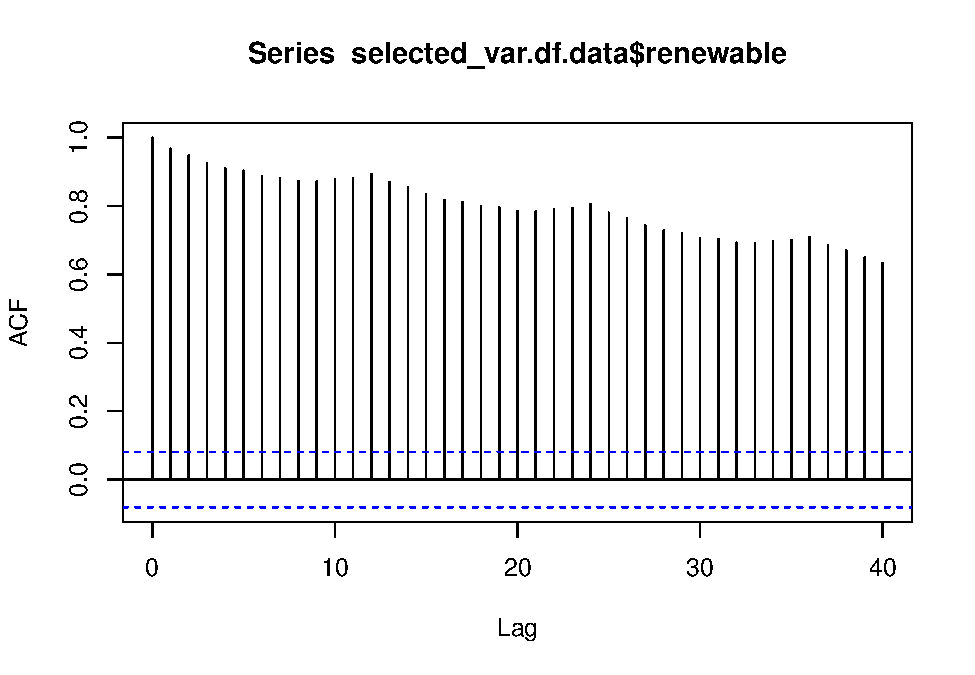
\includegraphics{YaredAsfaw_TSA_A02_Sp22_files/figure-latex/unnamed-chunk-19-1.pdf}

\hypertarget{overall-the-correlation-between-the-observations-of-the-total-renewable-energy-production-at-different-time-series-is-significant-but-show-a-decreasing-trend-as-the-time-lag-increase.}{%
\subsubsection{Overall the correlation between the observations of the
total renewable energy production at different time series is
significant but show a decreasing trend as the time lag
increase.}\label{overall-the-correlation-between-the-observations-of-the-total-renewable-energy-production-at-different-time-series-is-significant-but-show-a-decreasing-trend-as-the-time-lag-increase.}}

\begin{Shaded}
\begin{Highlighting}[]
\NormalTok{acf\_ts.hyd\_usage }\OtherTok{\textless{}{-}} \FunctionTok{acf}\NormalTok{(selected\_var.df.data}\SpecialCharTok{$}\NormalTok{hydro, }\AttributeTok{lag.max =} \DecValTok{40}\NormalTok{, }\AttributeTok{plot=}\ConstantTok{TRUE}\NormalTok{) }
\end{Highlighting}
\end{Shaded}

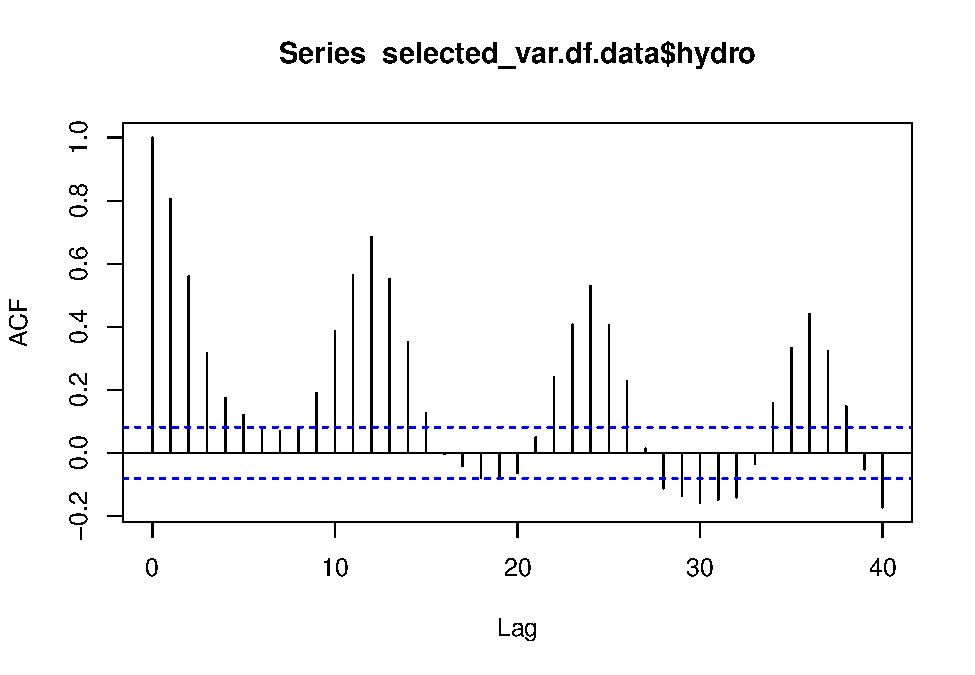
\includegraphics{YaredAsfaw_TSA_A02_Sp22_files/figure-latex/unnamed-chunk-20-1.pdf}

\hypertarget{overall-the-correlation-between-the-observations-of-the-the-hydroelectric-power-consumption-show-a-noticeable-decreasing-trend-for-the-first-10-lag-and-then-starts-to-increase-following-a-kind-of-normal-distribution-slightly-increasing-reach-at-peak-and-then-decline-again-slightly-for-the-times-the-observations-are-available.}{%
\subsubsection{Overall the correlation between the observations of the
the hydroelectric power consumption show a noticeable decreasing trend
for the first 10 lag and then starts to increase following a kind of
normal distribution (slightly increasing, reach at peak and then decline
again slightly) for the times the observations are
available.}\label{overall-the-correlation-between-the-observations-of-the-the-hydroelectric-power-consumption-show-a-noticeable-decreasing-trend-for-the-first-10-lag-and-then-starts-to-increase-following-a-kind-of-normal-distribution-slightly-increasing-reach-at-peak-and-then-decline-again-slightly-for-the-times-the-observations-are-available.}}

\hypertarget{the-first-two-plots-the-total-biomass-energy-production-and-the-total-renewable-energy-production-nearly-have-the-same-trend-with-slightly-different-behaviours.-however-the-third-plot-the-hydroelectric-power-plot-has-completely-different-behaviour-from-the-other-two-plots.}{%
\subsubsection{The first two plots (the total biomass energy production
and the total renewable energy production) nearly have the same trend
with slightly different behaviours. However, the third plot (the
hydroelectric power plot) has completely different behaviour from the
other two
plots.}\label{the-first-two-plots-the-total-biomass-energy-production-and-the-total-renewable-energy-production-nearly-have-the-same-trend-with-slightly-different-behaviours.-however-the-third-plot-the-hydroelectric-power-plot-has-completely-different-behaviour-from-the-other-two-plots.}}

\hypertarget{question-7}{%
\subsection{Question 7}\label{question-7}}

Compute the partial autocorrelation function from lag 1 to lag 40 for
these three variables. How these plots differ from the ones in Q6?

\begin{Shaded}
\begin{Highlighting}[]
\NormalTok{pacf\_ts.biomass }\OtherTok{\textless{}{-}} \FunctionTok{pacf}\NormalTok{(selected\_var.df.data}\SpecialCharTok{$}\NormalTok{biomass, }\AttributeTok{lag.max =} \DecValTok{40}\NormalTok{, }\AttributeTok{plot=}\ConstantTok{TRUE}\NormalTok{)}
\end{Highlighting}
\end{Shaded}

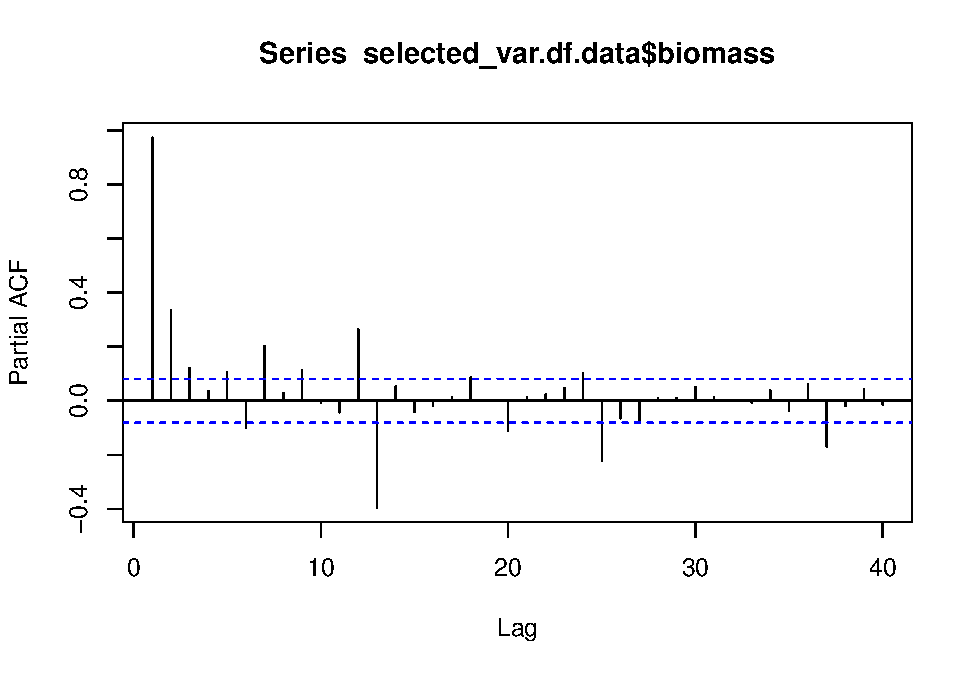
\includegraphics{YaredAsfaw_TSA_A02_Sp22_files/figure-latex/unnamed-chunk-21-1.pdf}

\hypertarget{looking-at-partial-autocorrelation-of-the-observations-of-the-total-biomass-energy-energy-production-from-lag-1-to-lag-40-there-is-significant-relationship-among-some-observations-until-lag-11-and-the-relationship-continue-to-fade-upon-moving-to-lag-40.}{%
\subsubsection{Looking at partial autocorrelation of the observations of
the total biomass energy energy production from lag 1 to lag 40, there
is significant relationship among some observations until lag 11 and the
relationship continue to fade upon moving to lag
40.}\label{looking-at-partial-autocorrelation-of-the-observations-of-the-total-biomass-energy-energy-production-from-lag-1-to-lag-40-there-is-significant-relationship-among-some-observations-until-lag-11-and-the-relationship-continue-to-fade-upon-moving-to-lag-40.}}

\begin{Shaded}
\begin{Highlighting}[]
\NormalTok{pacf\_ts.Re.energy }\OtherTok{\textless{}{-}} \FunctionTok{pacf}\NormalTok{(selected\_var.df.data}\SpecialCharTok{$}\NormalTok{renewable, }\AttributeTok{lag.max =} \DecValTok{40}\NormalTok{, }\AttributeTok{plot=}\ConstantTok{TRUE}\NormalTok{)}
\end{Highlighting}
\end{Shaded}

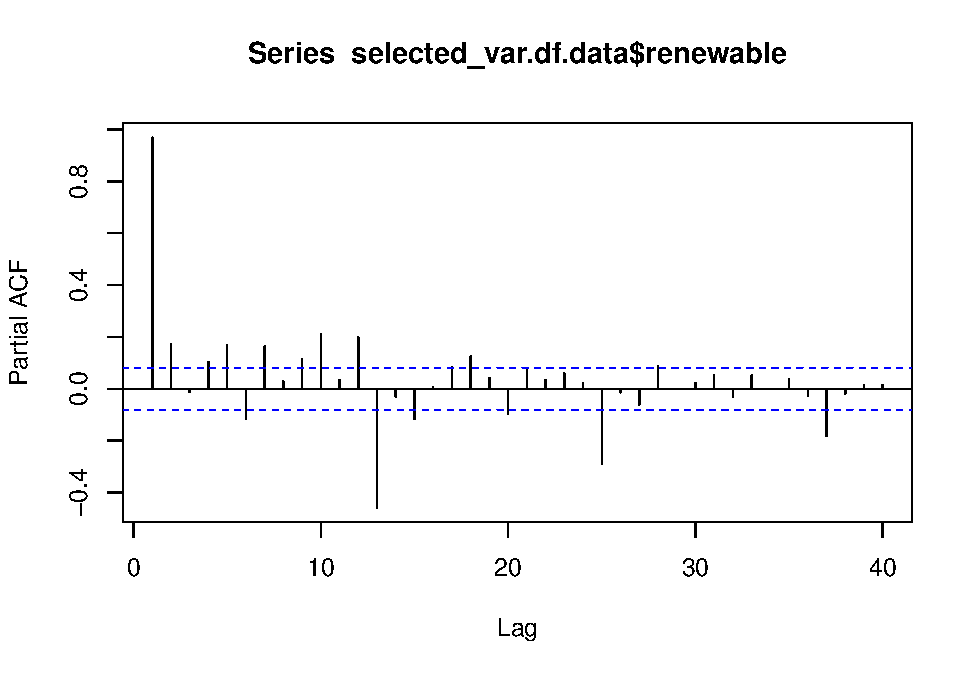
\includegraphics{YaredAsfaw_TSA_A02_Sp22_files/figure-latex/unnamed-chunk-22-1.pdf}

\hypertarget{looking-at-the-partial-aoutcorrelation-of-the-total-renewable-energy-production-observations-from-lag-1-to-lag-40-there-is-significant-relationship-among-some-observations-until-lag-11-and-the-relationship-continue-to-fade-upon-moving-to-lag-40.}{%
\subsubsection{Looking at the partial aoutcorrelation of the total
renewable energy production observations from lag 1 to lag 40, there is
significant relationship among some observations until lag 11 and the
relationship continue to fade upon moving to lag
40.}\label{looking-at-the-partial-aoutcorrelation-of-the-total-renewable-energy-production-observations-from-lag-1-to-lag-40-there-is-significant-relationship-among-some-observations-until-lag-11-and-the-relationship-continue-to-fade-upon-moving-to-lag-40.}}

\begin{Shaded}
\begin{Highlighting}[]
\NormalTok{pacf\_ts.hyd\_usage }\OtherTok{\textless{}{-}} \FunctionTok{pacf}\NormalTok{(selected\_var.df.data}\SpecialCharTok{$}\NormalTok{hydro, }\AttributeTok{lag.max =} \DecValTok{40}\NormalTok{, }\AttributeTok{plot=}\ConstantTok{TRUE}\NormalTok{)}
\end{Highlighting}
\end{Shaded}

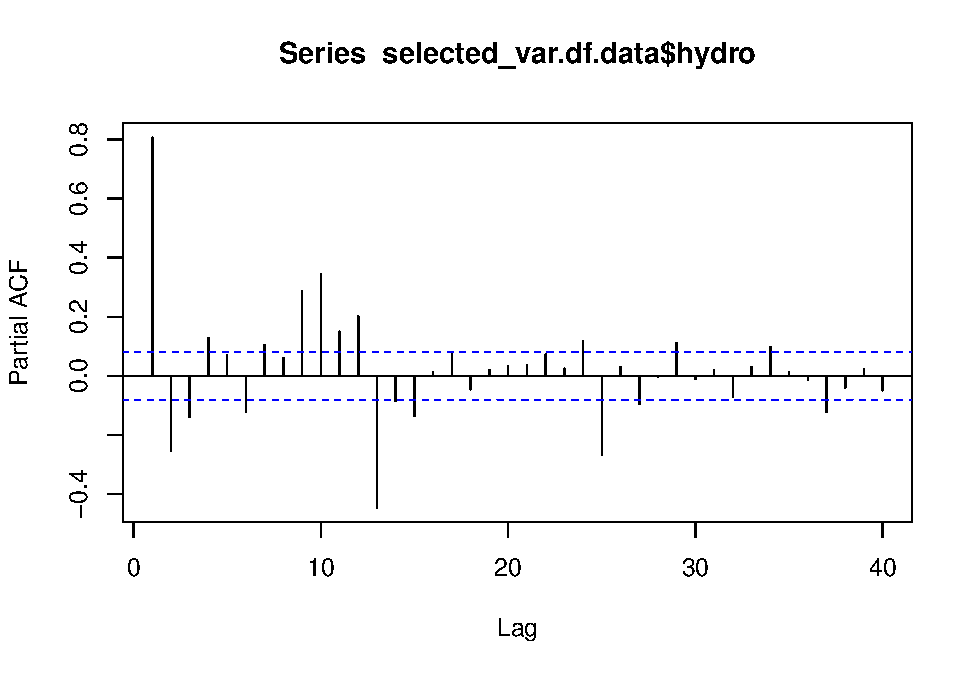
\includegraphics{YaredAsfaw_TSA_A02_Sp22_files/figure-latex/unnamed-chunk-23-1.pdf}

\hypertarget{looking-at-the-partial-aoutcorrelation-of-the-hydroelectric-power-consumption-observations-from-lag-1-to-lag-40-there-is-significant-relationship-among-some-observations-around-lag-9-and-10-only.}{%
\subsubsection{Looking at the partial aoutcorrelation of the
hydroelectric power consumption observations from lag 1 to lag 40, there
is significant relationship among some observations around lag 9 and 10
only.}\label{looking-at-the-partial-aoutcorrelation-of-the-hydroelectric-power-consumption-observations-from-lag-1-to-lag-40-there-is-significant-relationship-among-some-observations-around-lag-9-and-10-only.}}

\hypertarget{the-partial-autocorrelation-plots-differ-from-the-one-under-question-number-6-autocorrelation-plots-the-partial-autocorrelation-plots-use-the-first-and-40th-lags-by-ommitting-and-striping-out-any-infulence-between-the-two-data-points.}{%
\subsubsection{The partial autocorrelation plots differ from the one
under question number 6 (autocorrelation plots), the partial
autocorrelation plots use the first and 40th lags by ommitting and
striping out any infulence between the two data
points.}\label{the-partial-autocorrelation-plots-differ-from-the-one-under-question-number-6-autocorrelation-plots-the-partial-autocorrelation-plots-use-the-first-and-40th-lags-by-ommitting-and-striping-out-any-infulence-between-the-two-data-points.}}

\end{document}
